\section{守恒量与对称性}

\begin{quotation}
``对称性决定相互作用-扬振宁原理''
\end{quotation}

\begin{figure}[h]
\begin{center}
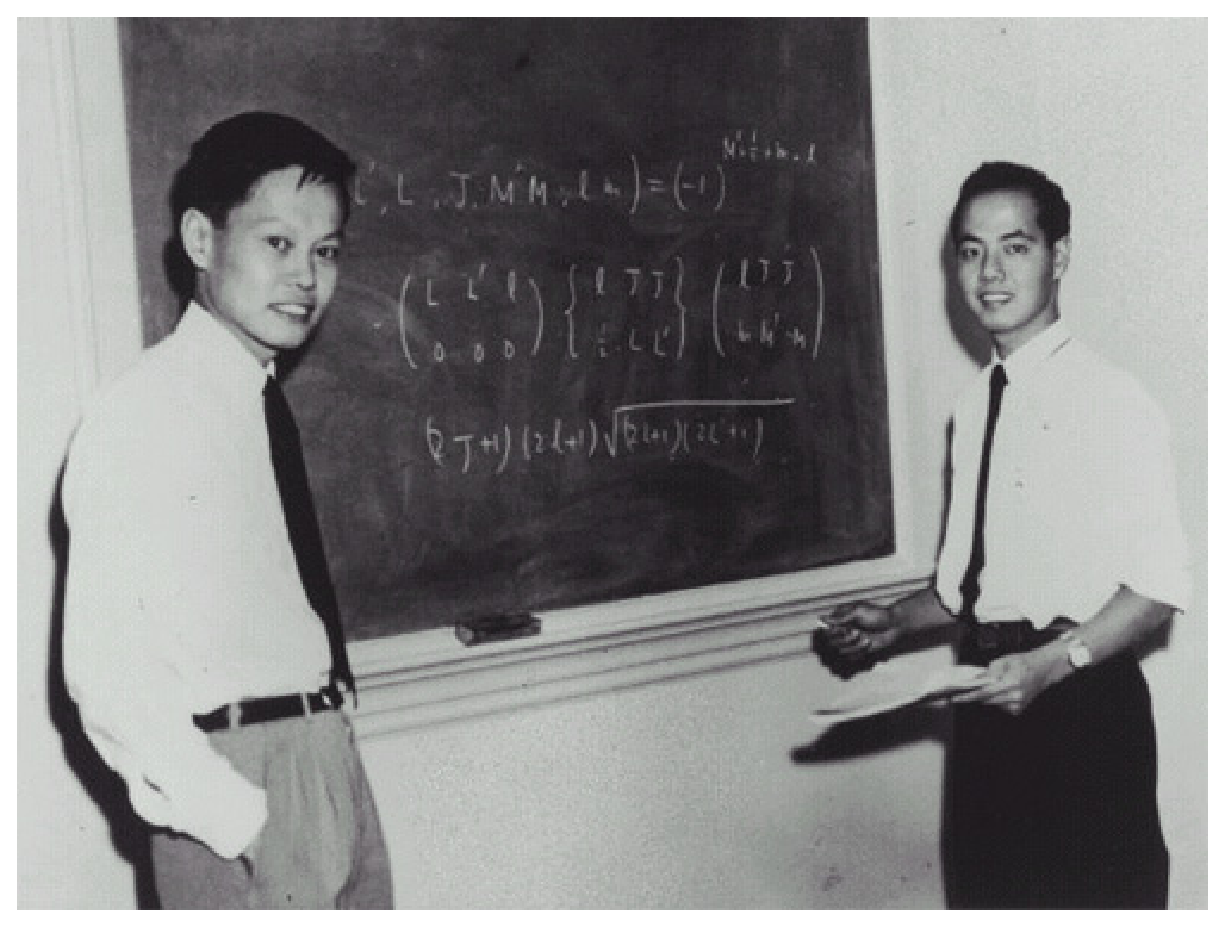
\includegraphics[clip,width=8cm]{Symmetry/yang-lee.ps}
\caption{杨振宁与李政道}
\end{center}
\end{figure}

\subsection{力学量随时间的变化}

力学量$F$在给定任意波函数$\psi$下的平均值:$\overline F  = \int {\psi ^* (x,t)\widehat F\psi (x,t)dx} $,随时间变化的关系:

\begin{equation}\label{16-1}
\frac{{d\overline F }}{{dt}} = \int {\frac{{\partial \psi ^* }}{{\partial t}}} \widehat F\psi dx + \int {\psi ^* \frac{{\partial \widehat F}}{{\partial t}}\psi dx}  + \int {\psi ^* \widehat F\frac{{\partial \psi }}{{\partial t}}dx}
\end{equation}

薛定谔方程:

\begin{equation}\label{16-2}
\widehat H\psi  = \widehat E\psi  = i\hbar \frac{\partial }{{\partial t}}\psi
\end{equation}

所以:$\frac{{\partial \psi }}{{\partial t}} = \frac{1}{{i\hbar }}\widehat H\psi $,在等式两边取复共厄:

\begin{center}
$\frac{{\partial \psi ^* }}{{\partial t}} =  - \frac{1}{{i\hbar }}\left( {\widehat H\psi } \right)^* $
\end{center}

方程\ref{16-1}化为:

\begin{equation}\label{16-3}
\frac{{d\overline F }}{{dt}} =  - \int {\frac{1}{{i\hbar }}\left( {\widehat H\psi } \right)} ^* \widehat F\psi dx + \int {\psi ^* \frac{{\partial \widehat F}}{{\partial t}}\psi dx}  + \int {\psi ^* \widehat F\frac{1}{{i\hbar }}\left( {\widehat H\psi } \right)dx}
\end{equation}

由于$\hat H$是厄密算符:$\int {\psi ^* \left( {\widehat H\varphi } \right)dx}  = \int {\left( {\widehat H\psi } \right)} ^* \varphi dx$,所以:

\begin{equation*}
\int {\left( {\widehat H\psi } \right)} ^* \widehat F\psi dx = \int {\psi ^* \widehat H\widehat F\psi dx} 
\end{equation*}

方程\ref{16-3}化为:

\begin{eqnarray*}
\frac{{d\overline F }}{{dt}} & = &  - \frac{1}{{i\hbar }}\int \psi  ^* \widehat H\widehat F\psi dx + \frac{1}{{i\hbar }}\int {\psi ^* \widehat F\widehat H\psi dx}  + \int {\psi ^* \frac{{\partial \widehat F}}{{\partial t}}\psi dx} \\
{}& = & \int {\psi ^* {\textstyle{{\left[ {\widehat F,\widehat H} \right]} \over {i\hbar }}}\psi dx}  + \int {\psi ^* \frac{{\partial \widehat F}}{{\partial t}}\psi dx} 
\end{eqnarray*}

即:

\begin{equation}\label{16-4}
\frac{{d\overline F }}{{dt}} = \overline {\frac{{\partial F}}{{\partial t}}}  + \frac{1}{{i\hbar }}\overline {\left[ {\widehat F,\widehat H} \right]}
\end{equation}

如果算符$\hat F$不显含时间,$\frac{{\partial \widehat F}}{{\partial t}} = 0$, $\frac{{d\overline F }}{{dt}} = \frac{1}{{i\hbar }}\overline {\left[ {\widehat F,\widehat H} \right]} $


如果算符$\hat F$不显含时间,而且算符$\hat F$与$\hat H$对易,$\frac{{d\overline F }}{{dt}} = 0$,即:力学量$\hat F$ 的平均值不随时间变化,称为守恒量;

在经典力学中我们用正则变量$q,p$描述系统运动状态,任何力学量均可表示为$q,p,t$的函数$F(q,p,t)$;力学量随时间变化的关系:


\begin{equation}\label{16-5}
\frac{{dF}}{{dt}} = \frac{{\partial F}}{{\partial t}} + \left( {\frac{{\partial F}}{{\partial q}}\dot q + \frac{{\partial F}}{{\partial p}}\dot p} \right)
\end{equation}


由正则方程:$\dot q = \frac{{\partial H}}{{\partial p}}$, $\dot p =  - \frac{{\partial H}}{{\partial q}}$, 方程\ref{16-5}化为:

\begin{equation}\label{16-6}
\frac{{dF}}{{dt}} = \frac{{\partial F}}{{\partial t}} + \left( {\frac{{\partial F}}{{\partial q}}\frac{{\partial H}}{{\partial p}} - \frac{{\partial F}}{{\partial p}}\frac{{\partial H}}{{\partial q}}} \right)
\end{equation}

引入泊松括号(Poisson bracket):

\index{Poisson bracket: 泊松括号}

\begin{equation}\label{16-7}
\left\{ {F,H} \right\} = \frac{{\partial F}}{{\partial q}}\frac{{\partial H}}{{\partial p}} - \frac{{\partial F}}{{\partial p}}\frac{{\partial H}}{{\partial q}}
\end{equation}

方程\ref{16-6}化为:

\begin{equation}\label{16-8}
\frac{{dF}}{{dt}} = \frac{{\partial F}}{{\partial t}} + \left\{ {F,H} \right\}
\end{equation}

可见经典运动方程\ref{16-8}与量子运动方程\ref{16-4}在形式上是类似的。

\textbf{守恒量的例子:}\footnote{参考周士勋《量子力学教程》第96页}

(1)自由粒子的动量:$\frac{{d\overline p }}{{dt}} = \frac{1}{{i\hbar }}\overline {\left[ {\widehat p,\widehat H} \right]}  = 0$

(2)中心力场中的动量:$\frac{{d\overline {L^2 } }}{{dt}} = \frac{1}{{i\hbar }}\overline {\left[ {\widehat L^2 ,\widehat H} \right]}  = 0$

(3)量子力学中的能量守恒:$\frac{{d\overline H }}{{dt}} = \frac{1}{{i\hbar }}\overline {\left[ {\widehat H,\widehat H} \right]}  = 0$

(4)宇称守恒定律:

空间反演变换:

\index{Space inversion: 空间反演}

\begin{equation}\label{16-9}
\widehat P\psi \left( {x,t} \right) = \psi \left( { - x,t} \right)
\end{equation}

$\hat P$:宇称算符,宇称算符的本征方程:$\widehat P\psi \left( {x,t} \right) = \lambda \psi \left( {x,t} \right)$

\index{Parity: 宇称}

\begin{center}
$\widehat P^2 \psi \left( {x,t} \right) = \widehat P\psi \left( { - x,t} \right) = \psi \left( {x,t} \right) = \lambda ^2 \psi \left( {x,t} \right)$
\end{center}

所以:$\widehat P^2 $的本征值是1;$\hat P$的本征值是$ \pm 1$;

$\hat P$的本征值是1的波函数:具有偶宇称的波函数;$\hat P$的本征值是-1的波函数:具有奇宇称的波函数;

假设哈密顿算符$\hat H$在空间反演变化下不变:$\widehat P\widehat H(x) = \widehat H( - x) = \widehat H(x)$;

\begin{center}
$\widehat P\widehat H(x)\psi (x,t) = \widehat H( - x)\psi ( - x,t) = \widehat H(x)\widehat P\psi (x,t)$
\end{center}

即:$\left[ {\widehat P,\widehat H} \right] = 0$,哈密顿算符$\hat H$与宇称算符$\hat P$对易;所以宇称是守恒量,$\hat H$和$\hat P$可以有共同本征函数;

\textbf{例1:}证明宇称算符是厄密算符;

\index{Hermitian operator: 厄米算符}

$\widehat P\psi (x) = \psi ( - x)$, $\left( {\widehat P\psi (x)} \right)^*  = \psi ^* ( - x)$

积分:

$\int_{ - \infty }^\infty  {\psi ^* (x)\widehat P\varphi (x)dx}  = \int_{ - \infty }^\infty  {\psi ^* (x)\varphi ( - x)dx}  = \int_{ - \infty }^\infty  {\left( {\widehat P^ +  \psi (x)} \right)^* \varphi (x)dx} $

积分变换:$x \to  - x$,

$\int_{ - \infty }^\infty  {\psi ^* (x)\varphi ( - x)dx}  =  - \int_\infty ^{ - \infty } {\psi ^* ( - x)\varphi (x)dx}  = \int_{ - \infty }^\infty  {\psi ^* ( - x)\varphi (x)dx}  = \int_{ - \infty }^\infty  {\left( {\widehat P\psi (x)} \right)^* \varphi (x)dx} $

比较积分变换前后的积分式,$\widehat P^ +   = \widehat P$,问题得证。


\subsection{对称变换}

假设变换$\hat Q$不含$t$, 使波函数:$\psi ' = \widehat Q\psi
$;并存在逆变换$\widehat Q^{ - 1} $: $\psi = \widehat Q^{ - 1} \psi
' = \widehat Q^{ - 1} \widehat Q\psi $ 变换后的波函数$\psi
'$与变换前的波函数$\psi$都满足薛定谔方程:

$\widehat H\psi  = i\hbar \frac{\partial }{{\partial t}}\psi $, $\widehat H\psi ' = i\hbar \frac{\partial }{{\partial t}}\psi '$

即:$\widehat H\widehat Q\psi  = i\hbar \frac{\partial }{{\partial t}}\widehat Q\psi $, 左乘逆变换$\widehat Q^{ - 1} $

$\widehat Q^{ - 1} \widehat H\widehat Q\psi  = i\hbar \frac{\partial }{{\partial t}}\psi  = \widehat H\psi $, 所以: $\widehat Q^{ - 1} \widehat H\widehat Q = \widehat H$

即:$\widehat H\widehat Q = \widehat Q\widehat H$, $\left[ {\widehat Q,\widehat H} \right] = 0$

满足$\widehat Q^{ - 1} \widehat H\widehat Q = \widehat H$的变换就是对称变换;$\hat Q$不一定是厄密算符,所以$\hat Q$ 本身并不一定是守恒量;考虑变换前后概率守恒:$\left( {\psi ,\psi } \right) = \left( {\widehat Q\psi ,\widehat Q\psi } \right) = \left( {\widehat Q^ +  \widehat Q\psi ,\psi } \right)$,即:$\widehat Q^ +  \widehat Q = \widehat 1$;所以$\hat Q$是幺正算符,或说$\hat Q$是幺正变换;

物理学中的对称变换总是构成一个群,称为对称群,在量子力学中也称为薛定谔群;

\index{Group: 群}

\index{Schrodinger group: 薛定谔群}

\textbf{群的定义:}设有一系列元素$G = \left\{ {a,b,c,...} \right\}$的集合,在它们之间定义了一种运算,姑且称之为``乘法'',并且满足以下性质:

\begin{enumerate}
    \item 封闭性: 若$a \in G$,$b \in G$,则其乘积$ab \in G$;
    \item 结合律: $(ab)c = a(bc)$;
    \item 存在单位元: 存在单位元素$e$,使对$G$内任一元素$a$,满足:$ae = ea = a$;
    \item 存在逆元: 对任一元素$a \in G$,存在一个元素$b \in G$,使$ba = ab = e$,$b$叫$a$的逆,记为:$a^{ - 1} $;
   \end{enumerate}

$\hat Q$可以是连续变换(如:平移,旋转),也可以是分立变换(空间反演,时间反演);对于连续变换,我们可以定义无穷小变换:$\widehat Q = 1 + i\varepsilon \widehat F$,$\varepsilon  \to 0 + $,要求$\hat Q$是幺正变换:

$\widehat Q^ +  \widehat Q = \left( {1 - i\varepsilon \widehat F^ +  } \right)\left( {1 + i\varepsilon \widehat F} \right) = 1 + i\varepsilon \left( {\widehat F - \widehat F^ +  } \right) + O\left( {\varepsilon ^2 } \right) = 1$,$O\left( {\varepsilon ^2 } \right) \to 0$

所以:$\widehat F^ +   = \widehat F$,即连续变换$\hat Q$可以表示为厄密算符$\hat F$的函数,$\hat F$:连续变换$\hat Q$ 的无穷小算子;由于$\hat F$是厄密算符,所以可以用$\hat F$定义一个与连续变换$\hat Q$相联系的力学量。由于$\left[ {\widehat Q,\widehat H} \right] = 0$,所以$\left[ {\widehat F,\widehat H} \right] = 0$,所以可以用来定义一个与对称变换$\hat Q$ 相关的守恒量。


\textbf{对称性决定守恒量的例子:}

(1)平移不变性与动量守恒:系统具有平移不变性,考虑平移变换,

\index{Momentum Conservation: 动量守恒}

\index{Translational invariance: 平移不变性}

$\widehat T:x' = x + \delta x$, $\delta x \to 0$无穷小位移;

波函数:$\widehat T:\psi ' = \widehat T\psi $, 平移不变:$\psi '(x') = \psi (x)$

$\widehat T\psi (x') = \widehat T\psi (x + \delta x) = \psi (x)$, 即:$\widehat T\psi (x) = \psi (x - \delta x)$

级数展开:

\begin{eqnarray*}
\widehat T\psi (x) & = & \psi (x - \delta x) = \psi (x) - \delta x\frac{{\partial \psi }}{{\partial x}} + \left( {\delta x} \right)^2 \frac{{\partial ^2 \psi }}{{\partial x^2 }} - ... \\
{} & = & \exp \left( { - \delta x\frac{{\partial \psi }}{{\partial x}}} \right)\psi (x) =
 \exp \left( { - \frac{{i\delta x}}{\hbar }\frac{\hbar }{i}\frac{{\partial \psi }}{{\partial x}}} \right)\psi (x) \\
 {} & = & \exp \left( { - \frac{{i\delta x\widehat p_x }}{\hbar }} \right)\psi (x) 
\end{eqnarray*}



动量算符:$\widehat p_x  = \frac{\hbar }{i}\frac{\partial }{{\partial x}}$是空间平移的无穷小算子;

系统具有平移不变性:$\widehat T^{ - 1} \widehat H\widehat T = \widehat H$, $ \Rightarrow \left[ {\widehat T,\widehat H} \right] = 0$, $ \Rightarrow \left[ {\widehat p_x ,\widehat H} \right] = 0$,即动量守恒;

(2)旋转不变性与角动量守恒:

\index{Rotational invariance: 旋转不变性}

系统具有球对称性,考虑旋转不变性。绕固定轴($z$轴)的转动:$\widehat R:\mathord{\buildrel{\lower3pt\hbox{$\scriptscriptstyle\rightharpoonup$}}
\over r} ' = \widehat R\mathord{\buildrel{\lower3pt\hbox{$\scriptscriptstyle\rightharpoonup$}}
\over r} $, 即:

\begin{center}
$\left( {\begin{array}{*{20}c}
   {x'}  \\
   {y'}  \\
\end{array}} \right) = \left( {\begin{array}{*{20}c}
   {\cos \varphi } & { - \sin \varphi }  \\
   {\sin \varphi } & {\cos \varphi }  \\
\end{array}} \right)\left( {\begin{array}{*{20}c}
   x  \\
   y  \\
\end{array}} \right)$
\end{center}

考虑无穷小变换(Infinitesimal transformation):$\varphi  \to \delta
\varphi  \to 0 + $, $\cos \delta \varphi  \to 1$, $\sin \delta
\varphi  \to \delta \varphi $

\index{Infinitesimal transformation: 无穷小变换}

\begin{center}
$\left( {\begin{array}{*{20}c}
   {x'}  \\
   {y'}  \\
\end{array}} \right) = \left( {\begin{array}{*{20}c}
   1 & { - \delta \varphi }  \\
   {\delta \varphi } & 1  \\
\end{array}} \right)\left( {\begin{array}{*{20}c}
   x  \\
   y  \\
\end{array}} \right)$
, 即:$\left\{ \begin{array}{l}
 x' = x - \delta \varphi y \\
 y' = \delta \varphi x + y \\
 \end{array} \right.$
\end{center}

波函数:$\widehat R\psi \left( {x,y} \right) = \psi \left( {x',y'} \right)$

\begin{eqnarray*}
\psi \left( {x',y'} \right) & = & \psi \left( {x - \delta \varphi y,y + \delta \varphi x} \right) \\
{} &=& \psi \left( {x,y} \right) - \delta \varphi y\frac{{\partial \psi \left( {x,y} \right)}}{{\partial x}} + \delta \varphi x\frac{{\partial \psi \left( {x,y} \right)}}{{\partial y}} + O(\delta \varphi ^2 ) \\
{} & = & \psi \left( {x,y} \right) + \delta \varphi \left( {x\frac{\partial }{{\partial y}} - y\frac{\partial }{{\partial x}}} \right)\psi \left( {x,y} \right) \\
{} &= & \psi \left( {x,y} \right) + \frac{{i\delta \varphi }}{\hbar }\frac{\hbar }{i}\left( {x\frac{\partial }{{\partial y}} - y\frac{\partial }{{\partial x}}} \right)\psi \left( {x,y} \right) \\
{} & = & \psi \left( {x,y} \right) + \frac{{i\delta \varphi \widehat L_z }}{\hbar }\psi \left( {x,y} \right) 
\end{eqnarray*}

因此:

\begin{equation*}
\widehat R_z  = 1 + \frac{{i\delta \varphi \widehat L_z }}{\hbar }
\end{equation*}


角动量算符:

\begin{equation}
\widehat L_z  = x\widehat p_y  - y\widehat p_x  = \frac{\hbar }{i}\left( {x\frac{\partial }{{\partial y}} - y\frac{\partial }{{\partial x}}} \right)
\end{equation}

是定$z$轴旋转的无穷小算子。

\index{Angular momentum: 角动量}

系统具有旋转不变性:$\widehat R^{ - 1} \widehat H\widehat R = \widehat H$, $ \Rightarrow \left[ {\widehat R,\widehat H} \right] = 0$, $ \Rightarrow \left[ {\widehat L_z ,\widehat H} \right] = 0$,即角动量守恒;类似我们还可定义$\widehat L_x $, $\widehat L_y $。

(3)时间平移不变性:

\index{Time-translation invariance: 时间平移不变性}

$i\hbar \frac{{\partial \psi }}{{\partial t}} = \widehat H\psi $, $\hat H$不显含时间。

$\psi (t) = \psi (0)e^{ - i{\textstyle{{\widehat Ht} \over \hbar }}} $,$t = \delta t \to 0$,$\psi (t) = \psi (0)\left( {1 - i\frac{{\widehat H\delta t}}{\hbar }} \right)$

时间无穷小平移算符是$\hat H$,对应有能量守恒。
